\scanpage{59}\mspage{58}
figures ensemblistes de t.f. \deleted{\unsure{que|qui}}\unsure{dont}
les multistrates sont dans $\deleted{\unsure{\mathcal F|F}}M$.

\uline{Remarque} En dehors du cas \inserted{finiment} spacieux, le
seul \inserted{autre} cas \unsure{intéressant} que j'ai rencontré
jusqu'à présent, est celui où la
relation $\underset{M}{\mathrel{\tikz[baseline=-.45ex,x=1em,y=1em]{\draw[line width=.055em] (.52,.27)--(.05,.055)--(.48,-.11); \draw[line width=.055em] (.14,.21)--(.46,.04)--(0,-.17);}}}$ est celle-ci : $X$ et $Y$
sont ensemblistement compatibles, et
$X\cap Y$ est \deleted{\unsure{un, une|une, une}} \inserted{ou bien vide, ou bien} élémentaire i.e.
est une multistrate commune.

Dans ce cas, $\mathcal F$ a la propriété
supplémentaire \unsure{intéressant|intéressante}
\begingroup\makeatletter\tagsleft@true\makeatother
\[
\begin{aligned}[t]
&\forall F\in\mathcal F,\quad \widetilde F\ \text{admet le inf de deux éléments}\\
&\text{\deleted{\unsure{i.e. tout}} \inserted{ou ce} qui revient au } = :\ \text{si } X,Y\in\deleted{\unsure{\mathcal F|F}}\widetilde F,\\
&\text{alors }\ X\cap Y\ \deleted{\unsure{\text{est}}}\ (\text{le inf pour }{\leq})\ \text{est}\\
&\text{encore une multistrate.}
\end{aligned}
\tag*{(\unsure{1,57|1.57})}
\]
\endgroup

\figure{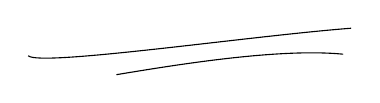
\begin{tikzpicture}[x=1cm,y=1cm]
\draw (0,0.06) .. controls (0.15,-0.08) and (2.8,0.31) .. (4.1,0.41);
\draw (1.12,-0.18) .. controls (1.9,-0.05) and (3.2,0.16) .. (4.0,0.08);
\end{tikzpicture}}
